\documentclass{standalone}
\usepackage{tikz}
\usepackage{amsmath}
\usepackage{circuitikz}
\begin{document}

%\begin{circuitikz}[scale=1.6]
%\draw[thick] (0,0) 
%    to[R,*-] (2,0)
%    to[L,*-] (2,1)
%    to[R,*-] (0,1) 
%    to[L,*-] (0,0)
%    to[R,*-] (-2,0)
%    to[L,*-] (-2,1)
%    to[R,*-] (0,1);
%\draw[thick] (2,1)  to[out=135,in=0] (0.1,1.825);
%\draw[thick] (-2,1) to[out=45,in=180] (-0.1,1.825);
%\draw[thick] (0.1,1.825)
%   to[C] (-0.1,1.825);
%
%\node (1) at (-2.5,0.5) {$N:$};
%\node (2) at (2.8,0.5) {};
%
%\end{circuitikz}

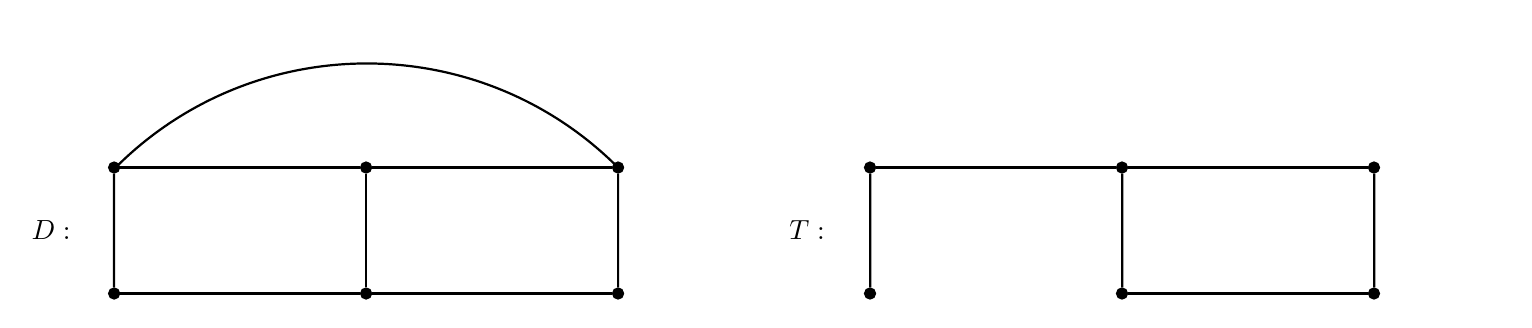
\begin{tikzpicture}[scale=1.6, inner sep=0.5mm, place/.style={circle,draw,fill}]
\draw[thick] (2,1) arc (45:135:2.82);
\node[place] (v1) at (0,1) {};
\node[place] (v2) at (-2,1) {};
\node[place] (v3) at (2,1) {};
\node[place] (v4) at (0,0) {};
\node[place] (v5) at (-2,0) {};
\node[place] (v6) at (2,0) {};

\draw[thick]  (v1) edge (v2);
\draw[thick]  (v2) edge (v5);
\draw[thick]  (v1) edge (v3);
\draw[thick]  (v4) edge (v5);
\draw[thick]  (v4) edge (v6);
\draw[thick]  (v6) edge (v3);
\draw[thick]  (v4) edge (v1);
\node (1) at (-2.5,0.5) {$D:$};


\node[place] (v11) at (6,1) {};
\node[place] (v12) at (4,1) {};
\node[place] (v13) at (8,1) {};
\node[place] (v14) at (6,0) {};
\node[place] (v15) at (4,0) {};
\node[place] (v16) at (8,0) {};
\node (2) at (3.5,0.5) {$T:$};
\draw[thick]  (v11) edge (v12);
\draw[thick]  (v12) edge (v15);
\draw[thick]  (v11) edge (v13);
%\draw  (v4) edge (v5);
\draw[thick]  (v14) edge (v16);
\draw[thick]  (v16) edge (v13);
\draw[thick]  (v14) edge (v11);

\node (3) at (9,0.5) {};
\end{tikzpicture}

\end{document}